\begin{exercises}

\exercise 证明转动惯量的平行轴定理:绕任何轴的转动惯量,等于
绕通过质心且与该轴平行的轴的转动惯量,加上物体的总质量乘
以两轴间距的平方。用公式表示为
\begin{equation*}
    I = I _ { c } + m r ^ { 2 }
\end{equation*}

\exercise 证明适用于薄的平面刚体的垂直轴定理:一个平面刚体薄
板,对于垂直板面某轴的转动惯量,等于绕平面内与该垂直轴相
交的任意两个正交轴的转动惯量之和。用公式表示为
\begin{equation*}
    I _ { z } = I _ { x } + I _ { y }
\end{equation*}

\exercise ~(1) 证明一条质量为$ m $、长为$ l $的均匀细杆,绕通过其中
心且垂直于杆身的轴的转动惯量为
\begin{equation*}
    I _ { c } = \frac { 1 } { 1 2 } m l ^ { 2 }
\end{equation*}

(2)用平行轴定理证明这杆绕通过其一端且垂直于杆身的转
动惯量为$  I = \dfrac { 1 } { 3 } m l ^ { 2 }  $。

\exercise 证明边长分别为$ a $和$ b $的矩形薄板,绕通过其中心且垂直
于板面的轴的转动惯量为$ I _ { c } = \dfrac { 1 } { 1 2 } + m \left( a ^ { 2 } + b ^ { 2 } \right)  $,其中$ m $为板的质量。
% 312.jpg
\clearpage
\exercise 边长分别为$ a $和$ b $的矩形薄板,质量为$ m $。现在中间挖去
一个边长为$ c $的正方形。绕通过其几何中心且与板面垂直的轴的
转动惯量是多少?

\exercise 在上题中,如果中间挖去的不是正方形,而是一个半径为
$ r $的圆形,则转动惯量$ I $又为多少?

\exercise 两个小球的质量分别为$  m _ { 1 } = 4 0   $克和$  m _ { 2 } = 1 2 0   $克,固定在一
条质量可忽略的轻棒的两端,棒长$  l = 2 0   $厘米。分别求出这系统对
于下列两轴的转动惯量。

(1)通过细棒的中心且垂直于棒;

(2)通过系统的质心且垂直于棒。

\exercise 求质量为$ m $、内半径为$ R_1 $、外半径为$ R_2 $的中空圆柱体对它
的几何对称轴的转动惯量。

\exercise 求质量为$ m $、半径为$ R $的薄圆盘对通过其直径的轴的转动
惯量。

\exercise 求质量为$ m $、半径为$ R $、厚为$ h $的圆盘,对通过质心且平
行于盘面的轴的转动惯量。

\exercise 门的宽度为$ 0.8 $米,质量为$ 5 $公斤,用手在离门轴$ 0.7 $米
\begin{wrapfigure}[6]{r}{12em}
    \centering
    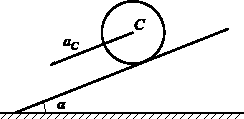
\includegraphics{figure/fig10.25}
    \caption{}
    \label{fig:10.25}
\end{wrapfigure}
处以$ 5.0 $牛顿的力推门,力的方
向与门的板面垂直,求门的角加
速度$ \beta $。

\exercise 一个均匀的球沿着与水
平面成$ \alpha $角的斜面无滑动地滚下
(图\ref{fig:10.25})  ,求球心的加速度$ \alpha $。

\exercise 一转动的飞轮,由于轴承摩擦力的作用,在$ 5 $秒钟内转
速由$ 900 $转/分减为$ 800 $转/分。求角加速度$ \beta $和$ 5 $秒内的转数问
再经几秒后飞轮停止转动?

\exercise 如图\ref{fig:10.26} 所示,在质量为$ M $、半径为$ R $的圆柱形滑轮上
缠绕细绳,绳一端挂有质量为$ m $的小物体,$ m $由高$ h $处从静止状态
% 313.jpg
下落。设绳不可伸长,滑轮与轴之间无摩擦。求$ m $达到地面时的
速度$ v $。
\begin{figure}[h]
    \begin{minipage}[b]{0.4\linewidth}
        \centering
        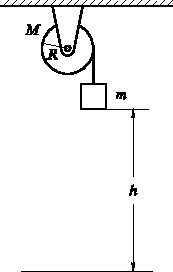
\includegraphics{figure/fig10.26}
        \caption{}
        \label{fig:10.26}
    \end{minipage}
    \begin{minipage}[b]{0.4\linewidth}
        \centering
        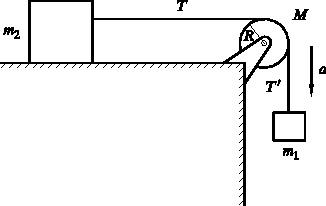
\includegraphics{figure/fig10.27}
        \caption{}
        \label{fig:10.27}
    \end{minipage}
\end{figure}

\exercise 如图\ref{fig:10.27} 中所示,质量为$  m _ { 1 }   $的物体以细绳绕过定滑轮
拉质量为$  m _ { 2 }   $的物体运动。滑轮半径为$ R $,质量为$ M $,其质量集中在
轮的边沿,$ m_2 $与平面间的摩擦系数为$ \mu $。设绳长不变,绳的质量
和滑轮与轴间的摩擦力都可略去不计。求绳中的张力$ T, T' $及$ m_1, m_2 $
的加速度$ a $。

\exercise 有一绕线圆盘,半径为$ R $,质量为$ m $,在其本身重量作用
下滚落,线的上端拴在天花板上,如图\ref{fig:10.28} 所示。求圆盘中心
\begin{wrapfigure}[8]{r}{13em}
    \centering
    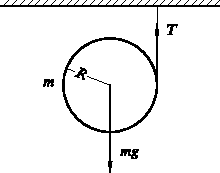
\includegraphics{figure/fig10.28}
    \caption{}
    \label{fig:10.28}
\end{wrapfigure}
下落的加速度$ a $和绳中的张力$ T $
(设绳不可伸长,绳质量可略去)。

\exercise 一质量为$ 10 $公斤,等分
$ 20 $级的梯子,以$ 60^\circ $的倾角架在
一面光滑的墙上,如图\ref{fig:10.29} 所
示。当一个体重为$ 60 $公斤的人沿
梯子向上爬到第$ 15 $级的时候,

\clearpage\noindent
% 314.jpg
\begin{wrapfigure}[12]{r}{11em}
    \centering
    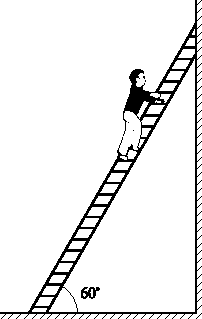
\includegraphics{figure/fig10.29}
    \caption{}
    \label{fig:10.29}
\end{wrapfigure}
梯子开始滑动,求这时地面给梯子的摩
擦力$  f  $。

\exercise 从高为$ h $的山顶上滚下一个
半径为R质量为$ m $的石滚子,只滚不
滑,求它到达山底时的速度$ v $。

\exercise 车床转速为$ 1,000 $转/分,功
率为$ 9.4 $千瓦,工作直径为$ 5.0 $厘米
问车刀克服的阻力f有多大?

\exercise 有一滑轮组如图\ref{fig:10.30} 所示,
两滑轮$ A $和$ B $的质量都是$ m $,半径都
是$ R $。滑轮$ A $可以随重物$ M $的下降而
上升。设绳子与滑轮之间无滑动,绳
长不变,绳子质量不计。分别求出$ M $下降的加速度$ a $和各段绳中
的张力$  T _ { 1 } , T _ { 2 } , T _ { 3 } $。

\begin{figure}[h]
    \begin{minipage}[b]{0.4\linewidth}
        \centering
        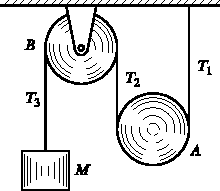
\includegraphics{figure/fig10.30}
        \caption{}
        \label{fig:10.30}
    \end{minipage}
    \begin{minipage}[b]{0.6\linewidth}
        \centering
        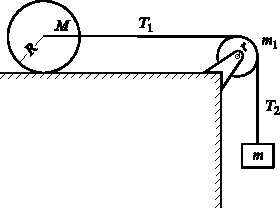
\includegraphics{figure/fig10.31}
        \caption{}
        \label{fig:10.31}
    \end{minipage}
\end{figure}

\exercise 一质量为$  M = 1 0   $公斤、半径为$  R = 2 0  $ 厘米的圆柱体,用绳
子系住它的轴,此绳跨过一质量为$  m _ { 1 } = 2 . 0   $公斤、半径为 $ r = 1 0   $厘
米的定滑轮,在绳的下端悬一质量为$  m = 5 . 0   $公斤的重物,如图
\ref{fig:10.31} 所示。设绳长不变,绳的质量及滑轮的轴间摩擦都可忽略
不计。当圆柱体沿桌面作纯滚动时,求:

% 315.jpg
\clearpage
(1) 重物的加速度$ a $;

(2) 绳的张力$  T _ { 1 } , T _ { 2 }  $。

\begin{wrapfigure}[8]{r}{11em}
    \vspace{-1em}
    \centering
    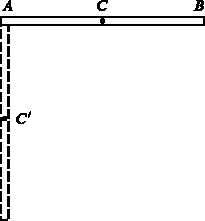
\includegraphics{figure/fig10.32}
    \caption{}
    \label{fig:10.32}
\end{wrapfigure}
\exercise 长为$ 2a $的匀质细棒$ AB $,以铰
链固结于$ A $点,起初它在水平位置静
止不动。当放开$ B $端,棒绕$ A $点转至
竖直位置时,铰链自动脱落,棒变为
自由落体。在以后的运动中,它的重
心$ C $走一抛物线抛迹,而棒本身则绕
重心$ C $转动试问当它的重心从$ C $位
置下降$ h $距离时,棒共转了几转?

\exercise 质量为$  k = 0 . 5 0$公斤的圆盘,直径为$  d = 4 0   $厘米,绕几何
轴转动;转速为$ n = 1,500 $转/分,欲使其在$  t = 2 0   $秒内停止,求制
动它的力矩。

\exercise 高为$  h = 5 . 0   $米的均匀细杆$ AB $,垂直插在地面上,因为根
部$ A $被锯断而倒向地面,求:

(1) 顶端$ B $到达地面时的线速度$ v_B $;

(2) 如果杆倒在地面时,它上面某点的速度恰如一物体从和
这点同样高度自由下落时的速度一样,求这点到$ A $点的距离$ y_H $。

\exercise 一个均匀球体和一个均匀圆柱体,具有相同的质量和半
径,沿同一斜面同时由静止开始向下动,只滚不滑,且起点在
同样的高度。哪个先到达下端?如果与一个无摩擦下滑的质点比
较,三者哪个下来得最快?哪个最慢?

\exercise 有以下四种球

(1)均匀实心钢球,半径为$  v = 5 .  0 $厘米;

(2)均匀实心塑料球,半径$  R = 1 0 . 0   $厘米;

(3)均匀钢球壳,半径$  r = 5 . 0   $厘米;

(4)均匀塑料球壳,半径$  R = 1 0 . 0   $厘米。\\
它们从同一斜面的同一高度$ h $同时由静止液下,斜面倾角为$ \alpha $,
% 316.jpg
球只滚不滑。求各球的质心加速度$  a _ { c }  $;各球到斜面底部时的速度
$ v _ { c }   $及球滚动的角速度。

\exercise 半径$  R = 1 0   $厘米、重量为$ P $的实心圆柱体以 $ \omega _ { 0 } = 1 0   $转/秒
的角速度绕几何轴旋转。把这个旋转着的圆柱体放到水平桌面
上,任其运动,于是它开始在桌面上连滚带滑。设圆柱体与桌面
间的滑动康擦系数为$  \mu = 0 . 1 0  $ 。问要经过多长时间$ t $后,圆柱体的
运动才能变成纯滚动?

\exercise 用手在不光滑的桌面上($  \mu \ne 0  $)  压一匀质的刚性球,使球
在桌面上开始连滚带滑,球心速度向右,速率为$  v _ { 0 }   $,球向左绕其质
心以$  \omega _ { 0 }   $旋转,如图\ref{fig:10.33} 所示。问 $ \omega _ { 0 }   $与$  v _ { 0 }   $之间满足什么条件,球
向右走了一段之后会向左滚着回来(这称之为“来去”)?又在什
么条件下,球会在向左行进的某时,同时停止又停转?再在什么
条件下,球会变为向右的纯滚动?

\begin{figure}[h]
    \begin{minipage}{0.4\linewidth}
        \centering
        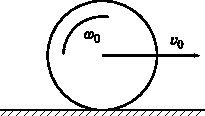
\includegraphics{figure/fig10.33}
        \caption{}
        \label{fig:10.33}
    \end{minipage}
    \begin{minipage}{0.6\linewidth}
        \centering
        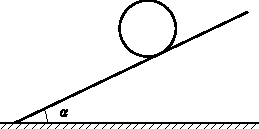
\includegraphics{figure/fig10.34}
        \caption{}
        \label{fig:10.34}
    \end{minipage}
\end{figure}

\exercise 一圆柱体从倾角为$ \alpha $的固定斜面上自由下落(图\ref{fig:10.34}) ,
斜面的摩擦系数至少应为多大,才会使圆柱体无滑动地纯滚动下
来?

\end{exercises}